\section{Diagnostics tools}
\label{section-diagnostics}

\curvgrid{} provides a diagnostics routine \textit{grid-diagnostics}, designed to analyze the grid construction procedure. As an example, consider running the routine on a 12 core machine, using a 4.2 million element first order \textit{Bullseye} mesh \cref{fig:result:bullseye}. The diagnostics routine uses \curvreader{}, \texttt{gridconstructor} and \curvwriter{} to read the mesh, construct the grid, and write the resulting grid into a VTU/PVTU file set. Afterwards, it runs a number of statistics tests, evaluating the element distribution, average size and curvature. \cref{fig:impl:storage:bullseyeelemdistr} presents the distribution of elements, process boundaries and domain boundaries among the 12 processes. At any point in time, \curvgrid{} can report parallel timing, that is, minimal and maximal time taken by each process for each timed stage of the grid (\cref{table:impl:storage:timelog}), using the \textit{LoggingTimer} utility. This utility can also be used to time user code. Finally, the \textit{RealTimeLog} utility, provided in \curvgrid{}, can be used to perform logging of the system memory real time by analyzing the corresponding system file. \cref{fig:impl:storage:realtimelog} presents the plot of the memory logging file, as it is output after the mesh has been written to file. By comparing the plot with the timing, one can discern that a large amount of extra memory is taken by auxiliary structures during the grid reading and writing. The grid construction is finished at 16:56:51, and takes $\approx$ 3.6 GB of total memory.

\begin{table}
\centering
\begin{tabular}{l l l}
\hline
	Min time [s]	& Max time [s]	& Action \\ \hline
	0.38411		& 0.384378	& CurvilinearGMSHReader: Skipping vertices \\
	3.86178		& 4.19604	& CurvilinearGMSHReader: Counting elements \\
	40.4335		& 40.7665	& CurvilinearGMSHReader: Reading and partitioning linear elements \\
	20.3694		& 23.1265	& CurvilinearGMSHReader: Reading complete element data \\
	11.071		& 13.6252	& CurvilinearGMSHReader: Reading boundary segment data \\
	0.758839	& 1.08354	& CurvilinearGMSHReader: Reading vertex coordinates \\
	3.50761		& 7.87511	& CurvilinearGMSHReader: Inserting entities into the factory \\
	8.29851		& 10.6347	& CurvilinearGridConstructor: Entity generation \\
	0.610859	& 2.95748	& CurvilinearGridConstructor: Global index generation \\
	0.228916	& 0.346936	& CurvilinearGridConstructor: Ghost element generation \\
	2.07785		& 2.81369	& CurvilinearGridConstructor: Index set generation \\
	0.300707	& 0.641833	& CurvilinearGridConstructor: Communication map generation \\
	0.0501765	& 0.685088	& CurvilinearGridConstructor: Communication of neighbor ranks \\
	151.23861	& 154.15874	& CurvilinearVTKWriter: Writing grid
\end{tabular}
\caption{\curvgrid{} parallel timing output for Bullseye grid diagnostics. Time is given in seconds. Minimum/maximum is taken over all processes doing the task}
\label{table:impl:storage:timelog}
\end{table}


\begin{figure}
\centering
	\begin{subfigure}[b]{0.48\textwidth} 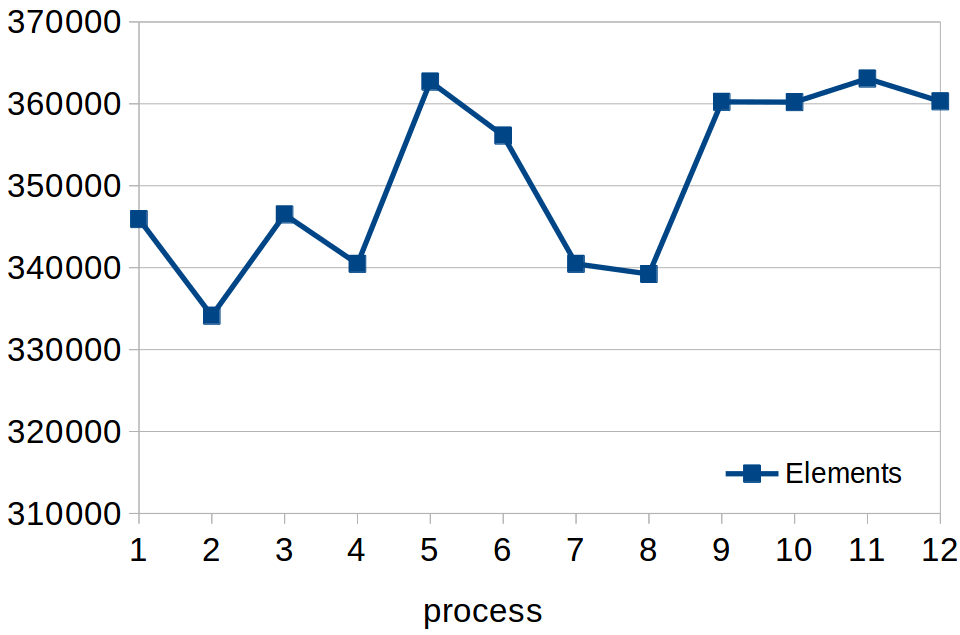
\includegraphics[scale=0.20]{images/elemdistr} \end{subfigure}
	\begin{subfigure}[b]{0.48\textwidth} 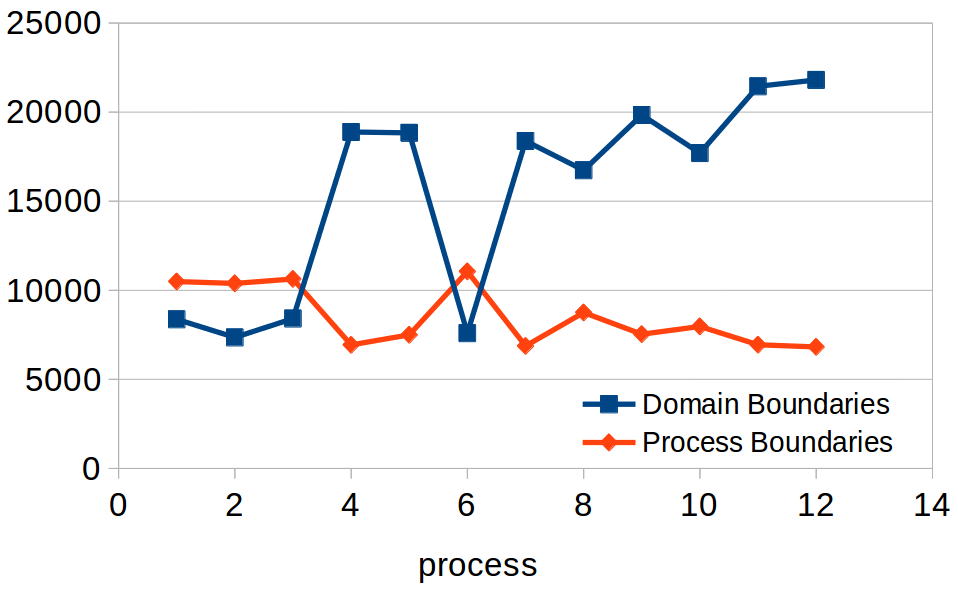
\includegraphics[scale=0.22]{images/boundarydistr} \end{subfigure}
\caption{Distribution of the Bullseye grid entities among 12 cores}
\label{fig:impl:storage:bullseyeelemdistr}
\end{figure}


\begin{figure}
\centering
	 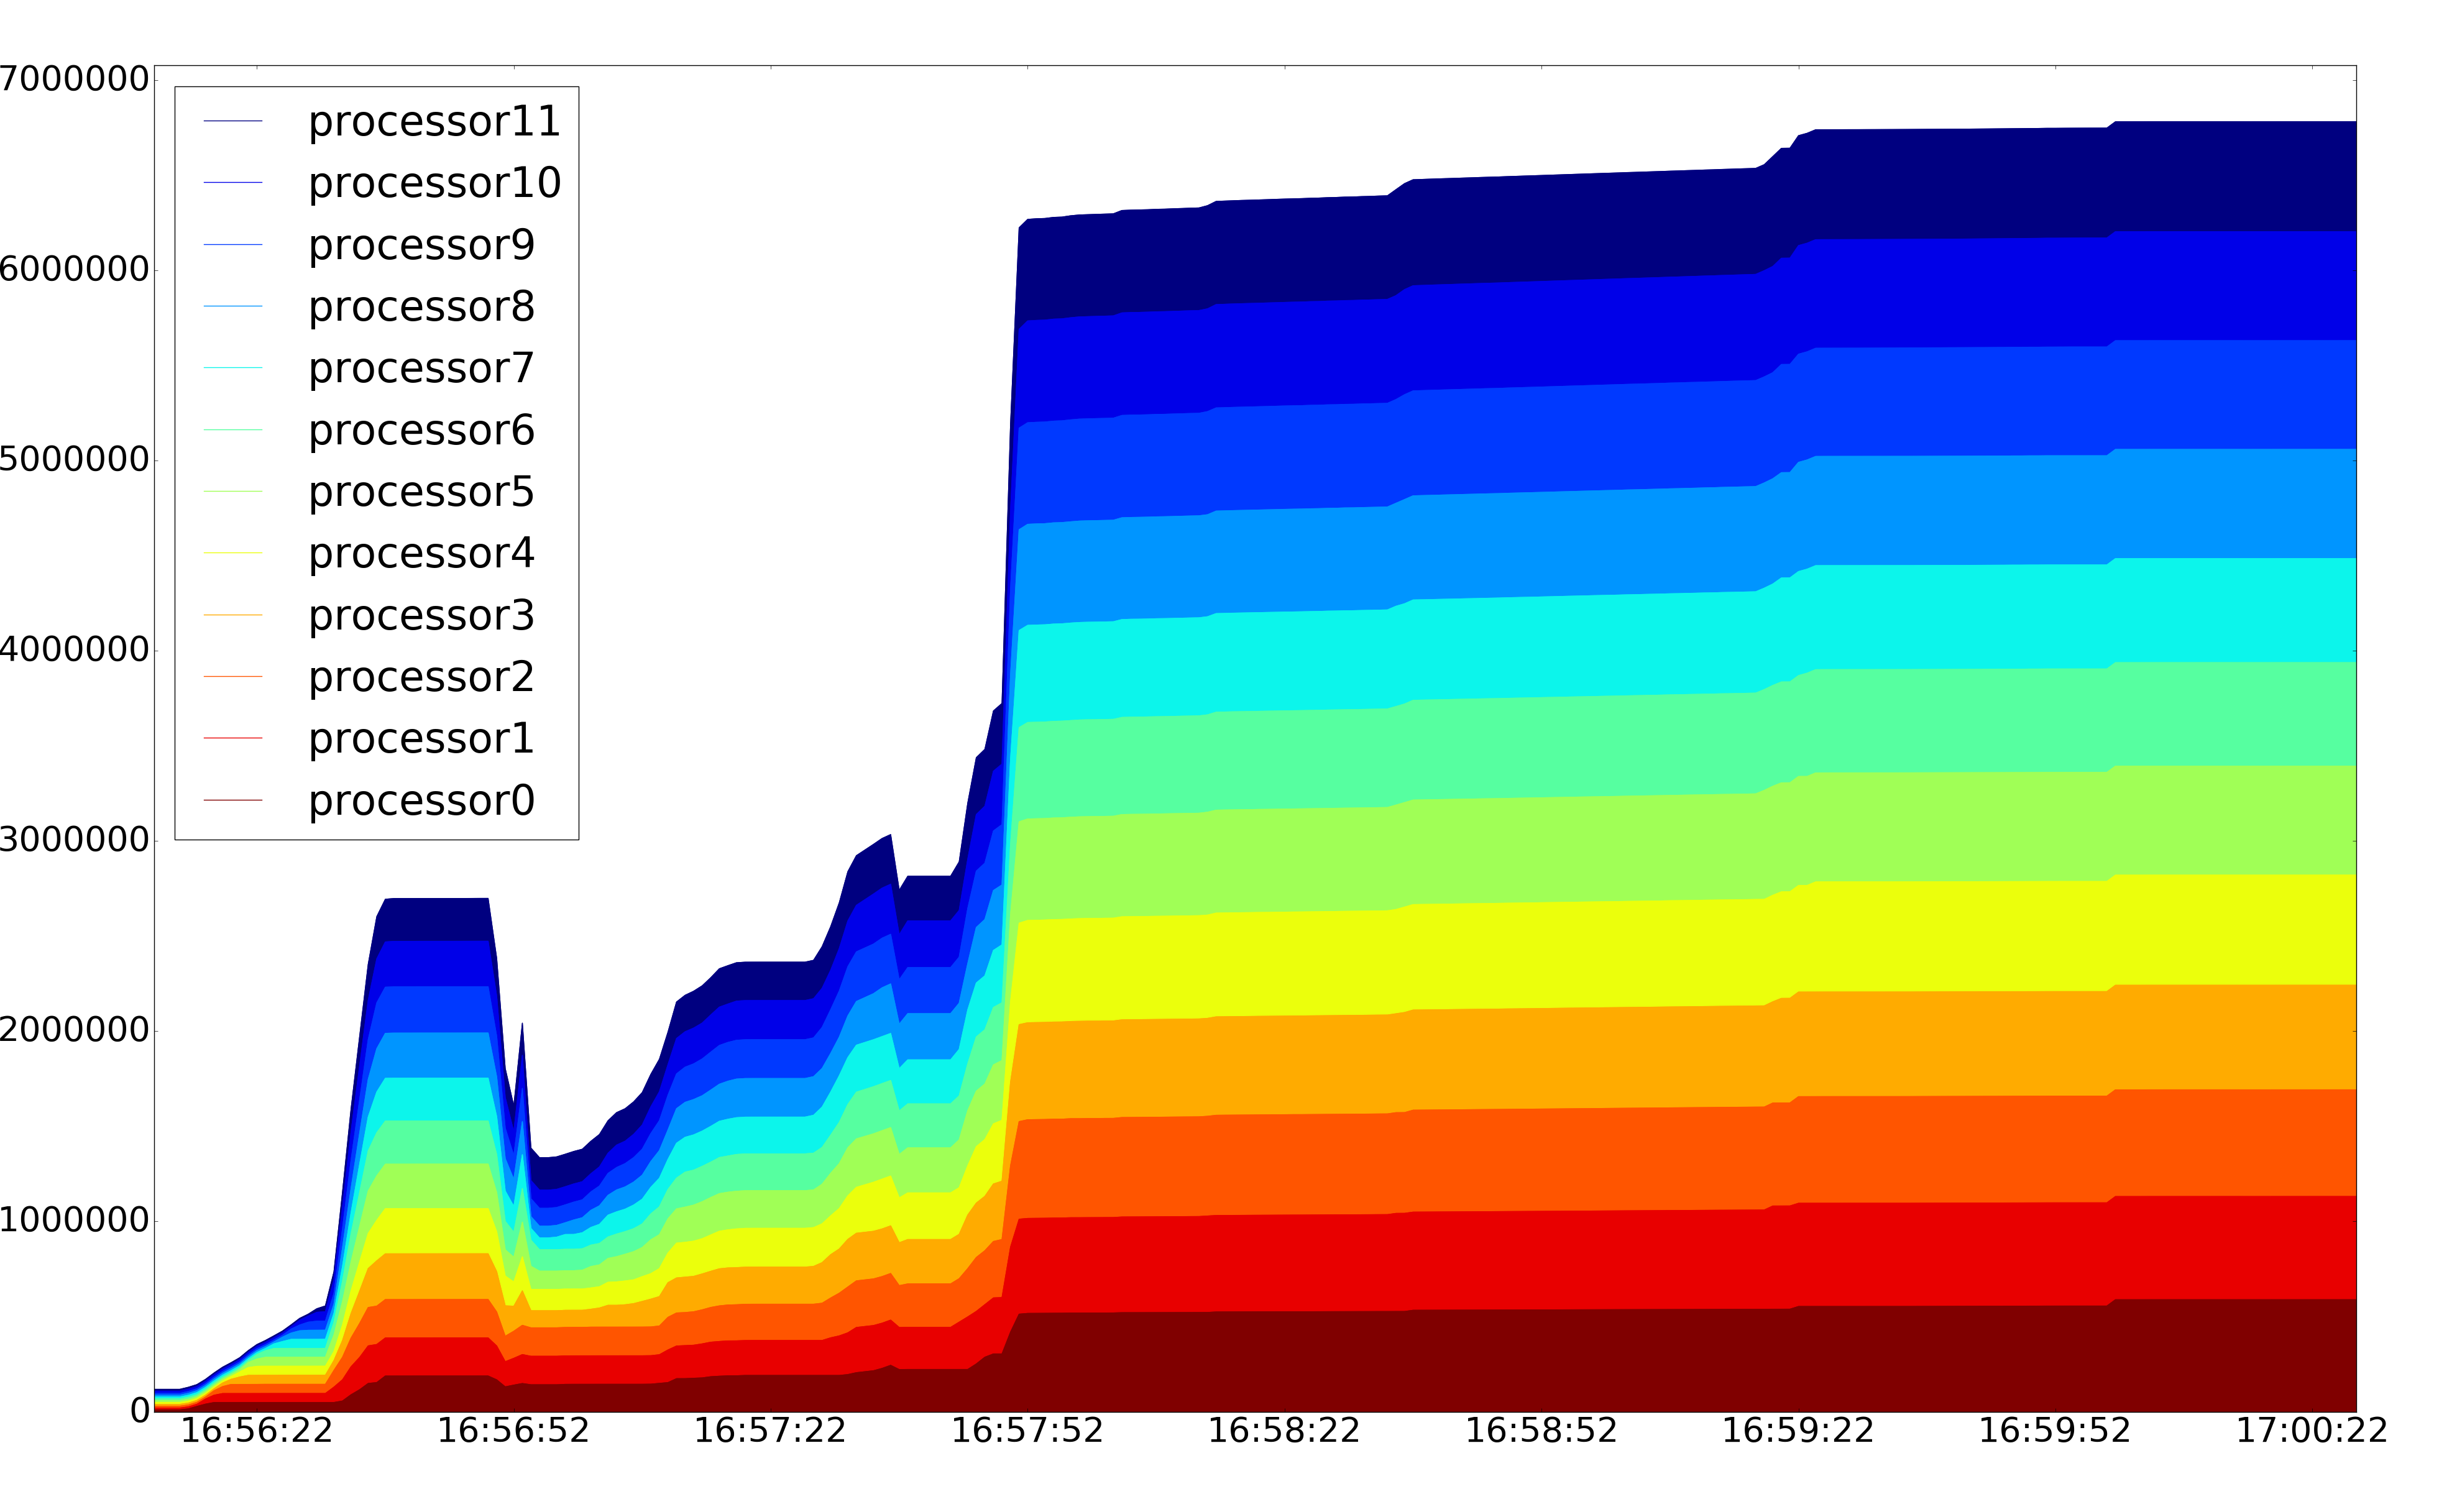
\includegraphics[scale=0.15]{images/realtimelog}
\caption{Memory consumption during the mesh reading, grid construction and writing. Memory is given in KB, and the curves are progressively added, meaning that the memory taken by each process corresponds to the area, not the absolute value. The x-axis corresponds to system time.}
\label{fig:impl:storage:realtimelog}
\end{figure}



% \subsection{Mesh statistics}
% \label{section-diagnostics-statistics}
% 
% 
% \subsection{Visualisation}
% \label{section-diagnostics-visualisation}